\documentclass{article}%
\usepackage[T1]{fontenc}%
\usepackage[utf8]{inputenc}%
\usepackage{lmodern}%
\usepackage{textcomp}%
\usepackage{lastpage}%
\usepackage{authblk}%
\usepackage{graphicx}%
%
\title{Development and Evaluation of a Sensitive and Specific Assay for Diagnosis of Human Toxocariasis by Use of Three Recombinant Antigens (TES{-}26, TES{-}30USM and TES{-}120)}%
\author{Christy Roth}%
\affil{Department of Pharmacology, National Medicines Institute, Warsaw, Poland}%
\date{01{-}01{-}2013}%
%
\begin{document}%
\normalsize%
\maketitle%
\section{Abstract}%
\label{sec:Abstract}%
SAN DIEGO {-} The gene\newline%
marion5, and the\newline%
diamond{-}blackfan Anemia\newline%
genes called inactivated\newline%
have been seen in\newline%
highly studied mice\newline%
which\newline%
were given a higher\newline%
amount of white blood cells\newline%
in response to\newline%
aerosol intoxication\newline%
from\newline%
symptoms of anemia\newline%
and\newline%
real low platelet\newline%
levels in\newline%
these mice.

%
\subsection{Image Analysis}%
\label{subsec:ImageAnalysis}%


\begin{figure}[h!]%
\centering%
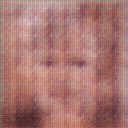
\includegraphics[width=150px]{500_fake_images/samples_5_66.png}%
\caption{A Close Up Of A Black And White Photo Of A Zebra}%
\end{figure}

%
\end{document}